\documentclass[main.tex]{subfiles}
\begin{document}
 
\section{Map Generation}

\par
The map is 16000 units wide and 9000 units high.
The maps are generated using a fixed set of rotated checkpoints $+-100$ units.

\lstset{caption={C++ code for map coordinates}}
\begin{lstlisting}
static vector<vector<Point>> maps =
{
  { {12460, 1350}, {10540, 5980}, {3580, 5180}, {13580, 7600} },
  { {3600, 5280}, {13840, 5080}, {10680, 2280}, {8700, 7460},
    {7200, 2160} },
  { {4560, 2180}, {7350, 4940}, {3320, 7230}, {14580, 7700}, 
    {10560, 5060}, {13100, 2320} },
  { {5010, 5260}, {11480, 6080}, {9100, 1840} },
  { {14660, 1410}, {3450, 7220}, {9420, 7240}, {5970, 4240} },
  { {3640, 4420}, {8000, 7900}, {13300, 5540}, {9560, 1400} },
  { {4100, 7420}, {13500, 2340}, {12940, 7220}, {5640, 2580} },
  { {14520, 7780}, {6320, 4290}, {7800, 860}, {7660, 5970},
    {3140, 7540}, {9520, 4380} },
  { {10040, 5970}, {13920, 1940}, {8020, 3260}, {2670, 7020} },
  { {7500, 6940}, {6000, 5360}, {11300, 2820} },
  { {4060, 4660}, {13040, 1900}, {6560, 7840}, {7480, 1360},
    {12700, 7100} },
  { {3020, 5190}, {6280, 7760}, {14100, 7760}, {13880, 1220},
    {10240, 4920}, {6100, 2200} },
  { {10323, 3366}, {11203, 5425}, {7259, 6656}, {5425, 2838} }
};
\end{lstlisting}

% \foreach \n in \checkpoints {
% $$n=\n$$
% }

\begin{figure}[h]
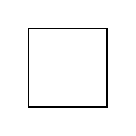
\begin{tikzpicture}
\draw (0, 0) rectangle (\sx{\mapwidth}, \sy{\mapheight});
\foreach [count=\i] \cpCount in \cpCounts {
    \foreach \j
        [evaluate={\j as \x using \checkpoints[\i - 1][\j - 1][0]}]
        [evaluate={\j as \y using \checkpoints[\i - 1][\j - 1][1]}]
        in {1,...,\cpCount} {
        \draw (\sx{\x}, \sy{\y}) circle [radius=\sx{\cpradius}];
        % \draw (\sx{12560}, \sy{1350}) -- (\sx{12560}, \sy{1350}) node {$0$};
    }
}
\end{tikzpicture}
\caption{All possible checkpoint placements}
\end{figure}

\section{All 13 possible maps}

\foreach [count=\i] \notUsed in \cpCounts {
% \foreach [count=\i] \cpCount in {4} {
\begin{center}
\begin{tikzpicture}
\drawmap{\i}
\end{tikzpicture}
\captionsetup{hypcap=false}
\captionof{figure}{Map Number: \i}\label{map\i}%
\end{center}
}
  
\end{document}

